\lstinputlisting[language=bash,basicstyle=\small]{python_codes/fieldstone_30/keywords.ascii}

\begin{center}
Code at \url{https://github.com/cedrict/fieldstone/tree/master/python_codes/fieldstone_30}
\end{center}

\par\noindent\rule{\textwidth}{0.4pt}
%%%%%%%%%%%%%%%%%%%%%%%%%%%%%%%%%%%%%%%%%%%%%%%%%%%%%%%%%%%%%%%%%%%%%%%%%%%%%%%%%%%%%%%%%%%5

In this \stone the Stokes equations are not solved and analytical 
velocity fields are used to advect particles. The CVI algorithm 
as introduced in Wang \etal (2015) \cite{waav15} is implemented.
Detailed derivations of the corrections and a thorough discussion 
of Wang \etal (2015) are presented in Section~\ref{MMM-sec:cvi}.
$Q_1$ and $Q_2$ basis functions are used and in both cases the CVI algorithm can be toggled on/off. 
Particles can be distributed regularly or randomly at startup.

Five velocity fields can be prescribed on the mesh:
\begin{itemize}
\item the so-called Couette flow of Wang \etal (2015) \cite{waav15} 
\item the SolCx solution (see Section~\ref{MMM-sec:geobench}, and  other stones too)
\item a flow created by means of a stream line function (see \stone 32)
\item a convection cell 
\item Donea \& Huerta manufactured solution, see Section~\ref{MMM-mms1}
\end{itemize}

The array {\python count} is {\python nel} long and contains the number of markers present in each element.
It is updated at every time step. Its min and max values are exported to an ascii file, as well 
as its standard deviation, computed with the {\python std} function of numpy defined as:
``The standard deviation is the square root of the average of the squared deviations from the mean, 
i.e., std = sqrt(mean(x)), where x = abs(a - a.mean())**2.''

Various Runge-Kutta algorithms (in space) are implemented, see Section~\ref{MMM-ss:rkm} and are 
controlled with the {\python RKorder} parameter.

%%%%%%%%%%%%%%%%%%%%%%%%%%%%%%%5
\subsection*{Couette flow}

\begin{center}
\includegraphics[width=7cm]{python_codes/fieldstone_30/results_couette/vel}\\
{\captionfont Velocity field - $32 \times 32$ $Q_1$ elements.}
\end{center}

\begin{center}
\includegraphics[width=4cm]{python_codes/fieldstone_30/results_couette/particles0000}
\includegraphics[width=4cm]{python_codes/fieldstone_30/results_couette/particles0010}
\includegraphics[width=4cm]{python_codes/fieldstone_30/results_couette/particles0020}\\
\includegraphics[width=4cm]{python_codes/fieldstone_30/results_couette/particles0030}
\includegraphics[width=4cm]{python_codes/fieldstone_30/results_couette/particles0040}
\includegraphics[width=4cm]{python_codes/fieldstone_30/results_couette/particles0050}
\end{center}

Due to the periodic boundary conditions, it only works with {\python RKorder}=1.

\newpage
%%%%%%%%%%%%%%%%%%%%%%%%%%%%%%%5
\subsection*{SolCx}

Reference model: $32\times 32$ resolution, CFL nb=0.5, $5^2$ particles randomly distributed inside each 
element, RKorder=2, $Q_1$ interpolation, no CVI.
We look at the min/max number of particles per element as a function of time (normalised 
by the initial number). Total of 500 time steps.

\begin{center}
\includegraphics[width=8cm]{python_codes/fieldstone_30/results_solcx/vel}\\
{\captionfont Velocity field - $32\times 32$ $Q_1$ elements.}
\end{center}

\begin{center}
\includegraphics[width=8cm]{python_codes/fieldstone_30/results_solcx/markercount_rk12345}
\includegraphics[width=8cm]{python_codes/fieldstone_30/results_solcx/stdev_rk12345}\\
{\captionfont Ref model + varying RKorder (the star means that velocity 
is directly computed on the particle, no interpolation).}
\end{center} 

\begin{center}
\includegraphics[width=8cm]{python_codes/fieldstone_30/results_solcx/markercount_q12}
\includegraphics[width=8cm]{python_codes/fieldstone_30/results_solcx/stdev_q12}\\
{\captionfont Ref model + $Q_1$ vs $Q_2$. }
\end{center}

\begin{center}
\includegraphics[width=8cm]{python_codes/fieldstone_30/results_solcx/markercount_npd}
\includegraphics[width=8cm]{python_codes/fieldstone_30/results_solcx/stdev_npd}\\
{\captionfont Ref model + initial nparticle per element between 4 and 8.}
\end{center}

\begin{center}
\includegraphics[width=8cm]{python_codes/fieldstone_30/results_solcx/markercount_cflnb}
\includegraphics[width=8cm]{python_codes/fieldstone_30/results_solcx/stdev_cflnb}\\
{\captionfont Ref model + CFL nb}
\end{center}

\begin{center}
\includegraphics[width=8cm]{python_codes/fieldstone_30/results_solcx/markercount_reg}
\includegraphics[width=8cm]{python_codes/fieldstone_30/results_solcx/stdev_reg}\\
{\captionfont Ref model + random vs regular.} 
\end{center}

\begin{center}
\includegraphics[width=8cm]{python_codes/fieldstone_30/results_solcx/markercount_res}
\includegraphics[width=8cm]{python_codes/fieldstone_30/results_solcx/stdev_res}\\
{\captionfont Ref model + different resolutions.}
\end{center}

Conclusion: nothing really helps, it is a matter of time before an element is fully depleted of particles. 
A regular distribution of markers makes things worse. Only using $Q_2$ interpolation seems to really do 
something. Using a small CFL number will improve things, but at the expense of the calculation walltime. 


\begin{center}
\includegraphics[width=8cm]{python_codes/fieldstone_30/results_solcx/markercount_cvi}
\includegraphics[width=8cm]{python_codes/fieldstone_30/results_solcx/stdev_cvi}\\
{\captionfont Ref model + influence of CVI.} 
\end{center}

We find that CVI makes a substantial difference. 


Coming back to the observations made in Section~\ref{MMM-sec:cvi}, 
we here show the $C_0$ quantity for three resolutions:

\begin{center}
\includegraphics[width=5cm]{python_codes/fieldstone_30/results_solcx/C0_16}
\includegraphics[width=5cm]{python_codes/fieldstone_30/results_solcx/C0_32}
\includegraphics[width=5cm]{python_codes/fieldstone_30/results_solcx/C0_64}\\
{\captionfont From left to right: 16x16, 32x32, 64x64.} 
\end{center}
We find that it becomes smaller and smaller, most likely in ${\cal O}(h)$.


\newpage
%%%%%%%%%%%%%%%%%%%%%%%%%%%%%%%5
\subsection*{Streamline flow}


\begin{center}
\includegraphics[width=8cm]{python_codes/fieldstone_30/results_streamline/vel}\\
{\captionfont 32x32 $Q_1$ mesh, 3x2 cells}
\end{center}

The reference model is as follows: 32x32 $Q_1$ elements, initial $5^2$ particles per element placed at random, 
CFL number of 0.5, RK order of 2, no CVI.
The {\tt count} array of length {\tt nel} is used to keep track of the number of particles per element. 
Its min/max values over time are recorded. The standard deviation of the {\tt count} array is also 
computed at each time step, normalised by the 
initial number of particles in the element at $t=0$ and plotted as a function of time. 

\begin{center}
\includegraphics[width=3.2cm]{python_codes/fieldstone_30/results_streamline/paint0001}
\includegraphics[width=3.2cm]{python_codes/fieldstone_30/results_streamline/paint0005}
\includegraphics[width=3.2cm]{python_codes/fieldstone_30/results_streamline/paint0010}
\includegraphics[width=3.2cm]{python_codes/fieldstone_30/results_streamline/paint0020}
\includegraphics[width=3.2cm]{python_codes/fieldstone_30/results_streamline/paint0050}\\
{\captionfont evolution of the swarm of markers.}
\end{center} 


\begin{center}
\includegraphics[width=8cm]{python_codes/fieldstone_30/results_streamline/markercount_rk12345}
\includegraphics[width=8cm]{python_codes/fieldstone_30/results_streamline/stdev_rk12345}\\
{\captionfont Ref model + varying RKorder (the star means that velocity 
is directly computed on the particle, no interpolation).}
\end{center} 

\begin{center}
\includegraphics[width=8cm]{python_codes/fieldstone_30/results_streamline/markercount_q12}
\includegraphics[width=8cm]{python_codes/fieldstone_30/results_streamline/stdev_q12}\\
{\captionfont Ref model + $Q_1$ vs $Q_2$. }
\end{center}

\begin{center}
\includegraphics[width=8cm]{python_codes/fieldstone_30/results_streamline/markercount_npd}
\includegraphics[width=8cm]{python_codes/fieldstone_30/results_streamline/stdev_npd}\\
{\captionfont Ref model + initial nparticle per element between 4 and 8.}
\end{center}

\begin{center}
\includegraphics[width=8cm]{python_codes/fieldstone_30/results_streamline/markercount_cflnb}
\includegraphics[width=8cm]{python_codes/fieldstone_30/results_streamline/stdev_cflnb}\\
{\captionfont Ref model + CFL nb}
\end{center}

\begin{center}
\includegraphics[width=8cm]{python_codes/fieldstone_30/results_streamline/markercount_reg}
\includegraphics[width=8cm]{python_codes/fieldstone_30/results_streamline/stdev_reg}\\
{\captionfont Ref model + random vs regular.} 
\end{center}

\begin{center}
\includegraphics[width=8cm]{python_codes/fieldstone_30/results_streamline/markercount_res}
\includegraphics[width=8cm]{python_codes/fieldstone_30/results_streamline/stdev_res}\\
{\captionfont Ref model + different resolutions.}
\end{center}

\begin{center}
\includegraphics[width=8cm]{python_codes/fieldstone_30/results_streamline/markercount_cvi}
\includegraphics[width=8cm]{python_codes/fieldstone_30/results_streamline/stdev_cvi}\\
{\captionfont Ref model + influence of CVI.}
\end{center}


In order to obtain the following figure no timestep is taken. The velocity is interpolated on 
the initial position of the markers (so is the CVI correction) and exported to a file along with 
the analytical value. The error for all markers is then presented in a histogram:
\begin{center}
\includegraphics[width=10cm]{python_codes/fieldstone_30/results_streamline/errors/histogram}\\
{\captionfont Distribution of velocity errors.}
\end{center}
We see that using CVI improves the accuracy of the velocity field error, but is no match for 
the results obtained with quadratic elements.

%%%%%%%%%%%%%%%%%%%%%%%%%%%%%%%%%%%%%%%%
\newpage
\subsection*{Convection in square domain}

In what follows I assume that the domain is the $[-1,1]\times[-1,1]$ square.
I postulate 
\begin{eqnarray}
u(x,y)&=&(a_0+a_1x+a_2x^2+a_3x^3+a_4x^4)(b_0+b_1y+b_2y^2+b_3y^3)\\
v(x,y)&=&(c_0+c_1y+c_2y^2+c_3y^3+c_4y^4)(d_0+d_1x+d_2x^2+d_3x^3)
\end{eqnarray}
I wish to enforce no flux through the boundaries so 
I need $u(\pm 1,y)=0$ and $v(x,\pm 1)=0$, so I choose 
\begin{eqnarray}
u(x,y)&=&(2-x^2-x^4)(b_0+b_1y+b_2y^2+b_3y^3)\\
v(x,y)&=&(2-y^2-y^4)(d_0+d_1x+d_2x^2+d_3x^3)
\end{eqnarray}
The velocity divergence is then
\begin{eqnarray}
\vec\nabla\cdot\vec\upnu =
-2(x+2x^3)(b_0+b_1y+b_2y^2+b_3y^3) -2 (y+2y^3)(d_0+d_1x+d_2x^2+d_3x^3) 
\end{eqnarray}
which yields:
\begin{eqnarray}
b_1+d_1&=&0 \\
b_3+2d_1 &=& 0 \\
2b_1 + d_3 &=& 0 \\
2b_3 + 2d_3 &=& 0
\end{eqnarray}
4 equations for 4 unknowns but we can only express three parameters
as a function of $d_1$:
\[
b_1=-d_1
\quad\quad
b_3=-2d_1
\quad\quad
d_3=2d_1
\]
I choose $d_1=1$ so finally
\begin{eqnarray}
u(x,y)&=&(2-x^2-x^4)(-y-2y^3) \\
v(x,y)&=&(2-y^2-y^4)( x+2x^3)
\end{eqnarray}
Let us quickly verify:
\[
\vec\nabla\cdot\vec\upnu =
(-2x-4x^3)(-y-2y^3) + (-2y-4y^3)(x+2x^3) = 
2(-x-2x^3)(-y-2y^3) + 2(-y-2y^3)(x+2x^3) = 0
\]

The computational domain remains the unit square, so we need to carry out 
a change of variables and the analytical velocity field inside the unit square is then 
\begin{eqnarray}
u(x,y)&=&(2-(2x-1)^2-(2x-1)^4)(-(2y-1)-2(2y-1)^3) \\
v(x,y)&=&(2-(2y-1)^2-(2y-1)^4)( (2x-1)+2(2x-1)^3)
\end{eqnarray}
This velocity field is shown hereunder:
\begin{center}
\includegraphics[width=7cm]{python_codes/fieldstone_30/results_box/vel}\\
{\captionfont Velocity field.}
\end{center}

\begin{center}
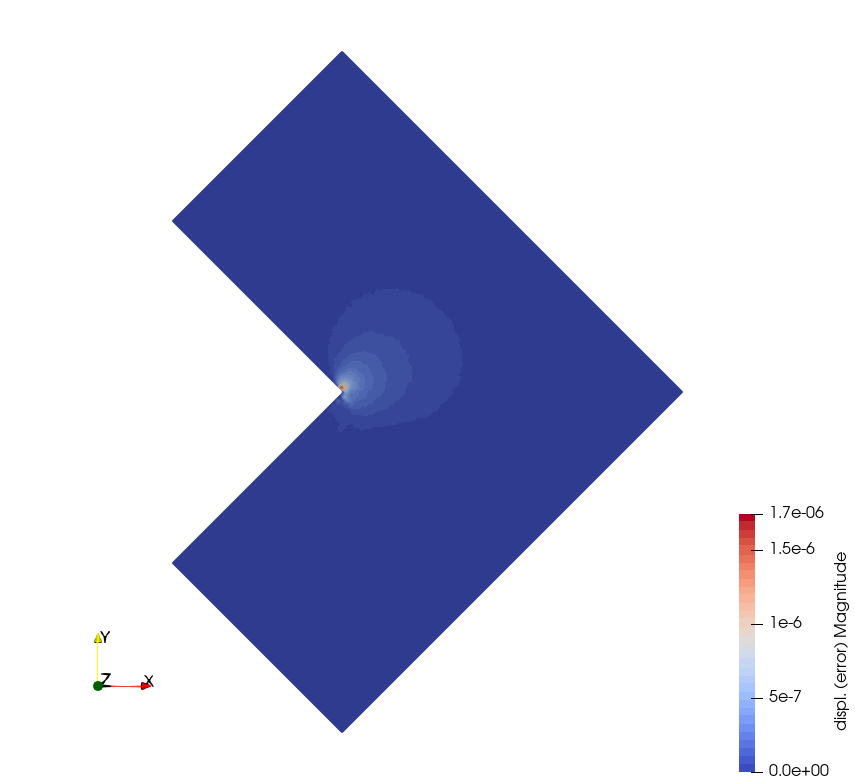
\includegraphics[width=5cm]{python_codes/fieldstone_30/results_box/error}
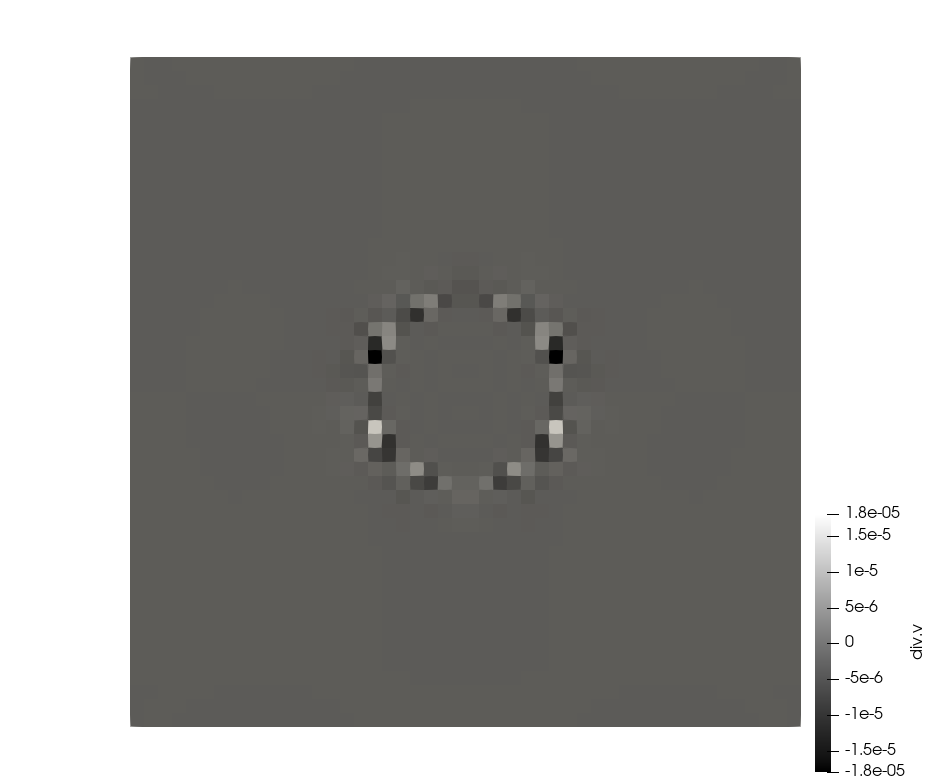
\includegraphics[width=5cm]{python_codes/fieldstone_30/results_box/divv}
\includegraphics[width=5cm]{python_codes/fieldstone_30/results_box/C0}\\
{\captionfont From left to right: velocity error (interpolated minus analytical),
velocity divergence, $C_0$ value. 64x64 mesh. } 
\end{center}
Note the difference between the amplitude of the velocity divergence and the $C_0$ term!

\begin{center}
\includegraphics[width=8cm]{python_codes/fieldstone_30/results_box/markercount_rk12345}
\includegraphics[width=8cm]{python_codes/fieldstone_30/results_box/stdev_rk12345}\\
{\captionfont Ref model + varying RKorder (the star means that velocity 
is directly computed on the particle, no interpolation).}
\end{center} 

\begin{center}
\includegraphics[width=8cm]{python_codes/fieldstone_30/results_box/markercount_q12}
\includegraphics[width=8cm]{python_codes/fieldstone_30/results_box/stdev_q12}\\
{\captionfont Ref model + $Q_1$ vs $Q_2$. }
\end{center}

\begin{center}
\includegraphics[width=8cm]{python_codes/fieldstone_30/results_box/markercount_npd}
\includegraphics[width=8cm]{python_codes/fieldstone_30/results_box/stdev_npd}\\
{\captionfont Ref model + initial nparticle per element between 4 and 8.}
\end{center}

\begin{center}
\includegraphics[width=8cm]{python_codes/fieldstone_30/results_box/markercount_cflnb}
\includegraphics[width=8cm]{python_codes/fieldstone_30/results_box/stdev_cflnb}\\
{\captionfont Ref model + CFL nb}
\end{center}

\begin{center}
\includegraphics[width=8cm]{python_codes/fieldstone_30/results_box/markercount_reg}
\includegraphics[width=8cm]{python_codes/fieldstone_30/results_box/stdev_reg}\\
{\captionfont Ref model + random vs regular.} 
\end{center}

\begin{center}
\includegraphics[width=8cm]{python_codes/fieldstone_30/results_box/markercount_res}
\includegraphics[width=8cm]{python_codes/fieldstone_30/results_box/stdev_res}\\
{\captionfont Ref model + different resolutions.}
\end{center}

\begin{center}
\includegraphics[width=8cm]{python_codes/fieldstone_30/results_box/markercount_cvi}
\includegraphics[width=8cm]{python_codes/fieldstone_30/results_box/stdev_cvi}\\
{\captionfont Ref model + influence of CVI.}
\end{center}

Despite similarities with SolCx (a convection cell in a rectangular domain),
advection without CVI does not yield areas with too little/many markers.
When CVI is used it does not alter results substantially.


%%%%%%%%%%%%%%%%%%%%%%%%%%%%%%%%%%%%%%%%
\newpage
\subsection*{Convection in square domain - Donea \& Huerta velocity field}

The domain is a unit square and the velocity field is the one of the 
Donea \& Huerta manufactured solution, see Section~\ref{MMM-mms1}:
\begin{eqnarray}
u(x,y) &=& x^2(1- x)^2 (2y - 6y^2 + 4y^3) = x^2(1-x)^2 2y (1-3y+2y^2) \nonumber\\
v(x,y) &=& -y^2 (1 - y)^2 (2x - 6x^2 + 4x^3) = -y^2 (1 - y)^2 2x (1-3x+2x^2) 
\end{eqnarray}

After a few hundreds of timesteps we find that 4 zones in the domain 
progressively contain less and less markers:

\begin{center}
\includegraphics[width=4.3cm]{python_codes/fieldstone_30/results_dh/count0000}
\includegraphics[width=4.3cm]{python_codes/fieldstone_30/results_dh/count0010}
\includegraphics[width=4.3cm]{python_codes/fieldstone_30/results_dh/count0040}
\includegraphics[width=4.3cm]{python_codes/fieldstone_30/results_dh/count0070}\\
\includegraphics[width=4.3cm]{python_codes/fieldstone_30/results_dh/mmm0000}
\includegraphics[width=4.3cm]{python_codes/fieldstone_30/results_dh/mmm0010}
\includegraphics[width=4.3cm]{python_codes/fieldstone_30/results_dh/mmm0040}
\includegraphics[width=4.3cm]{python_codes/fieldstone_30/results_dh/mmm0070}\\
{\captionfont Reference model.}
\end{center}

Looking at the marker count statistics we see that its minimum value reaches zero no 
matter what option is used, except for CVI: 

\begin{center}
\includegraphics[width=8cm]{python_codes/fieldstone_30/results_dh/markercount_rk12345}
\includegraphics[width=8cm]{python_codes/fieldstone_30/results_dh/stdev_rk12345}\\
{\captionfont Ref model + varying RKorder (the star means that velocity 
is directly computed on the particle, no interpolation).}
\end{center} 

\begin{center}
\includegraphics[width=8cm]{python_codes/fieldstone_30/results_dh/markercount_q12}
\includegraphics[width=8cm]{python_codes/fieldstone_30/results_dh/stdev_q12}\\
{\captionfont Ref model + $Q_1$, $Q_2$, $P_1$ and $P_2$. }
\end{center}

\begin{center}
\includegraphics[width=8cm]{python_codes/fieldstone_30/results_dh/markercount_npd}
\includegraphics[width=8cm]{python_codes/fieldstone_30/results_dh/stdev_npd}\\
{\captionfont Ref model + initial nparticle per element between 4 and 8.}
\end{center}

\begin{center}
\includegraphics[width=8cm]{python_codes/fieldstone_30/results_dh/markercount_cflnb}
\includegraphics[width=8cm]{python_codes/fieldstone_30/results_dh/stdev_cflnb}\\
{\captionfont Ref model + CFL nb}
\end{center}

\begin{center}
\includegraphics[width=8cm]{python_codes/fieldstone_30/results_dh/markercount_reg}
\includegraphics[width=8cm]{python_codes/fieldstone_30/results_dh/stdev_reg}\\
{\captionfont Ref model + random vs regular.} 
\end{center}

\begin{center}
\includegraphics[width=8cm]{python_codes/fieldstone_30/results_dh/markercount_res}
\includegraphics[width=8cm]{python_codes/fieldstone_30/results_dh/stdev_res}\\
{\captionfont Ref model + different resolutions.}
\end{center}

\begin{center}
\includegraphics[width=8cm]{python_codes/fieldstone_30/results_dh/markercount_cvi_Q1}
\includegraphics[width=8cm]{python_codes/fieldstone_30/results_dh/stdev_cvi_Q1}\\
{\captionfont Ref model + influence of CVI.}
\end{center}

\begin{center}
\includegraphics[width=8cm]{python_codes/fieldstone_30/results_dh/markercount_cvi_Q2}
\includegraphics[width=8cm]{python_codes/fieldstone_30/results_dh/stdev_cvi_Q2}\\
{\captionfont Ref model + $Q_2$ + influence of CVI.}
\end{center}

We can conclude that the cvi algorithm applied to $Q_2$ makes virtually no difference.
















